\documentclass[12pt,fleqn]{article}
%\usepackage {psfig,epsfig} % para incluir figuras em PostScript
\usepackage{amsfonts,amsthm,amsopn,amssymb,latexsym}
\usepackage{graphicx}
\usepackage[T1]{fontenc}
\usepackage[brazil]{babel}
\usepackage{geometry}
\usepackage[utf8]{inputenc}
\usepackage[intlimits]{amsmath}
\usepackage{listingsutf8}
\usepackage{float}
\usepackage{textcomp}
\usepackage{subcaption}
\lstdefinestyle{MatlabCustom}{
	language=Matlab,
	tabsize=4,
	showspaces=false,
	showstringspaces=false
}
\lstset{language=Matlab}
\lstset{inputencoding=utf8}
\lstset{basicstyle=\scriptsize,style=MatlabCustom}
\lstset{literate=%
{ó}{{\'{o}}}1
{å}{{\aa}}1
{Å}{{\AA}}1
{ç}{{\c{c}}}1
{ã}{{\~a}}1
}
\graphicspath{{./images/}}
%alguns macros
\newcommand{\R}{\ensuremath{\mathbb{R}}}
\newcommand{\Rn}{{\ensuremath{\mathbb{R}}}^{n}}
\newcommand{\Rm}{{\ensuremath{\mathbb{R}}}^{m}}
\newcommand{\Rmn}{{\ensuremath{\mathbb{R}}}^{{m}\times{n}}}
\newcommand{\contcaption}[1]{\vspace*{-0.6\baselineskip}\begin{center}#1\end{center}\vspace*{-0.6\baselineskip}}
%=======================================================================
\usepackage{a4}                       % tamanho da página
\setlength{\textwidth}{16.0cm}        % largura do texto
\setlength{\textheight}{9.0in}        % tamanho do texto (sem head, etc)
\renewcommand{\baselinestretch}{1.15} % espaçamento entre linhas
\addtolength{\topmargin}{-1cm}        % espaço entre o head e a margem
\setlength{\oddsidemargin}{-0.1cm}    % espaço entre o texto e a margem

% Ser indulgente no preenchimento das linhas
\sloppy

\begin{document}

\pagestyle {empty}

\vspace*{-2cm}
{\bf
\begin{center}
{\large
\hspace*{0cm}Universidade de São Paulo} \\
\hspace*{0cm}Escola Politécnica \\
\hspace*{0cm}Curso de Engenharia de Computação  \\
\end{center}}
\centerline{\includegraphics[scale=0.8]{logo-poli}}
\vspace{.5cm}
\noindent
\begin{center}
{\Large \bf Condução de calor em placa plana com fontes e sorvedouros} \\[2cm]
{\Large Tiago Koji Castro Shibata (8988730), tiago.shibata@usp.br}\\[6mm]
{\Large Deborah Hidemi Kamiguchi Watanabe (4430967), deborah.watanabe@usp.br}\\[6mm]
\vspace{.5cm}
\end{center}

{\raggedleft
\begin{minipage}[t]{8.0cm}
\setlength{\baselineskip}{0.25in}
RELATÓRIO apresentado ao Professor Alexandre Roma do MAP/IME-USP
como atividade da disciplina MAP3122 - Métodos Numéricos.
\end{minipage}\\[2cm]}

\vspace{1cm}
{\center São Paulo - SP \\[3mm]
31/03/2016 \\}

\newpage


\pagestyle {empty}
\abstract{Esse trabalho mostra modelos explícitos e implícitos de resolução da Equação Diferencial Parcial (EDP) de condução de calor para uma dimensão espacial (barra) e duas (placa), utilizando métodos numéricos aprendidos na disciplina MAP3122 - Métodos Numéricos e Aplicações.}

\newpage

\tableofcontents

% Numeração em romanos para páginas iniciais (sumários, listas, etc)
%\pagenumbering {roman}
\pagestyle {plain}

\setcounter{page}{0} \pagenumbering{arabic}

\setlength{\parindent}{0in}  %espaco entre paragrafo e margem
% Espaçamento entre parágrafos
\parskip 5pt
\newpage
\section{Introdução}
A geração de calor está presente no dia a dia de todos os seres. Desde as perdas de energias ocorrentes na mais simples das reações biológicas, o calor muitas vezes representa a energia desperdiçada, o movimento caótico de moléculas que se dispersam do fenômeno sendo realizado.

Na engenharia, a geração de calor e principalmente o aumento de temperatura têm grandes consequências, podendo criar um ambiente desagradável em uma construção mal planejada, queimar um motor ou causar danos em equipamentos. Em eletrônica, o aumento de temperatura leva circuitos a queimarem ou desligarem-se se possuírem proteção contra sobretemperatura. Neste trabalho, focamos em um modelo simples de condução de calor, em uma barra ou placa plana. A estrutura possuirá fontes e sorvedouros, simulando a ação de uma placa eletrônica metálica contendo componentes integrados. Algumas regiões (com componentes) serão tradadas como fontes de calor, e a placa como um todo terá uma pequena perda de calor (representando a troca de calor com o ar). Grande parte dos métodos e modelos são baseados no livro de Burden\&Faires~\cite{livro}.

Nesse trabalho, desejamos simular a condução de calor em uma barra ou placa a partir da equação de difusão de calor, aplicando métodos numéricos em soluções computacionais. Obteremos mapas de temperatura e fluxo de calor para diferentes condições e configurações. Apresentando a temperatura próxima aos componentes, podemos simular a temperatura na qual a placa final operará e tentar melhorar a disposição dos mesmos.

A seção ``Modelagem matemática'' descreve o modelo utilizado, indicando constantes relevantes à simulação. ``Metodologia de desenvolvimento'' relata como foi feito o desenvolvimento do trabalho. ``Métodos numéricos'' mostra detalhes do modelo, discretização utilizada e métodos aplicados. ``Resultados'' mostra verificações dos métodos e resultados adquiridos. Por espaço no relatório, o ordem de convergência será verificada pelo método das soluções manufaturadas apenas para um método (método explícito para barra). ``Conclusões'' fecha o relatório com conclusões pessoais dos autores.

\section{Modelagem matemática}
Em  nosso  modelo,  a  placa ou barra  será  discretizada  em  múltiplos  segmentos  de dimensão pequena. Cada pequeno segmento será a menor subdivisão que trataremos e possuirá uma temperatura homogênea.

As condições iniciais foram tomadas como temperatura homogênea em toda a extensão (componentes desligados e material em equilíbrio). A temperatura ambiente e inicial da placa foram tomadas como 0; assim, se um gráfico indica 30, significa que o material aqueceu 50\textdegree C em relação ao ambiente. O calor gerado é configurável, podendo ser colocado em diferentes posições e valores. Utiliza­-se o modelo de barra unidimensional/placa  bidimensional,  homogênea  e  isotrópica,  ou  seja,  suas propriedades não  se alteram em diferentes direções ou posições e a  condução térmica é constante em toda a sua extensão. Parâmetros do material necessários para o modelo são $k$ (condutividade térmica), $\rho$ (massa específica) e $c_p$ (calor específico).

Duas propriedades são de interesse nesse estudo: o fluxo de calor, que indica a passagem de energia térmica, é proporcional ao oposto do gradiente da temperatura. Estudos empiricos mostram que o fluxo de calor é proporcional à área de contato e à condutividade térmica \cite{ufsc_geracao_de_calor}:

\[q = -k A \frac{\partial u(x, t)}{\partial x} $ ou $ q = -k A \nabla u(x, y, t)\]
Onde $u$ representa a temperatura e $A$ a área de contato.

Observe que o modelo físico de fluxo de calor indica que ele flui do local mais quente para o menos quente (gradiente negativo). Além disso, e mais importante, é a temperatura nos pontos da barra. A equação de difusão de calor é:

\[\frac{\partial u(x, t)}{\partial t} = \alpha \frac{\partial^2 u(x, t)}{\partial x^2} + w(x) $ ou $ \frac{\partial u(x, y, t)}{\partial t} = \alpha \nabla^2 u(x, y, t) + w(x, y)\]

Sendo $\alpha$ chamado de coeficiente de difusão térmica e $w$ um calor recebido ou perdido externamente.

Observa-se que a equação relaciona a mudança  de  temperatura  em  certo  ponto  no  tempo  com  o  laplaciano  da temperatura, ou  o  divergente  do  gradiente,  representado  por  $\nabla$. Esse valor é intuitivo  e  semelhante  a  resultados  vistos  nas  disciplinas  de  física  e electromagnetismo:  o  aumento  de  temperatura  no  ponto  é  relacionado  com  o divergente  do  fluxo  de  calor,  ou  seja,  o  calor  realmente  “ganho”,  ficando  a temperatura  constante  se  calor  ganho de um lado é perdido para outro mais frio (ou seja, primeira derivada não nula, mas segunda derivada nula). Também  indica  que  um  ponto  pode  entrar  em  equilíbrio  térmico  mesmo  se  sua temperatura for diferente da temperatura em seu entorno, se seu “lucro” de calor for nulo.

A fórmula de condução de calor e o valor de $\alpha$ podem ser deduzidos a partir de outros parâmetros já citados. Em nosso modelo discretizado, podemos aproximar a derivada na interface entre dois blocos, ou seja, $\frac{\partial u(x - \frac{\Delta x}{2}, t)}{\partial x}$ e $\frac{\partial u(x + \frac{\Delta x}{2}, t)}{\partial x}$ (formas de aproximações serão mostradas na seção ``Métodos Numéricos''; por enquanto, assume-se que podemos calcular aproximações para esses valores). De posse desses valores aproximados, podemos aplicar expansão por polinômio de Taylor:

\[
\frac{\partial u(x + \frac{\Delta x}{2}, t)}{\partial x} = \frac{\partial u(x, t)}{\partial x} + \frac{\partial^2 u(x, t)}{\partial x^2} \frac{\Delta x}{2} + \frac{\partial^3 u(\xi_1, t)}{x^3} \frac{\Delta x^2}{8}, \xi_1 \in [x, x + \frac{\Delta x}{2}]
\]
\[
\frac{\partial u(x - \frac{\Delta x}{2}, t)}{\partial x} = \frac{\partial u(x, t)}{\partial x} - \frac{\partial^2 u(x, t)}{\partial x^2} \frac{\Delta x}{2} + \frac{\partial^3 u(\xi_2, t)}{x^3} \frac{\Delta x^2}{8}, \xi_2 \in [x - \frac{\Delta x}{2}, x]
\]

O ganho de calor é o ``lucro'' de calor, ou seja, a diferença entre o recebido de um lado e perdido de outro. Subtraíndo as equações acima e adicionando os termos $k$ e $A$ da equação de fluxo de calor, temos:

\[\Delta Q $ (calor ganho) $ = 2 k A \frac{\partial^2 u(x, t)}{\partial x^2} \frac{\Delta x}{2} = k A \frac{\partial^2 u(x, t)}{\partial x^2} \Delta x $, com $|erro| = |k A [ \frac{\partial^3 u(\xi_1, t)}{x^3} \frac{\Delta x^2}{8} - \frac{\partial^3 u(\xi_2, t)}{x^3} \frac{\Delta x^2}{8}]|\]

No entanto, diferentes objetos possuem diferentes capacidades térmicas (C), que indicam quanto calor é necessário para variar sua temperatura em um grau ($\Delta u = \frac{Q}{C}$). A capacidade térmica é diretamente proporcional à massa (ou seja, se a massa dobra, precisamos do dobro de energia para aquecê-la uma mesma quantidade). Um parâmetro melhor para representar materiais é o calor específico, que possui significado semelhante à capacidade térmica, mas é invariante à massa ($c_p = \frac{C}{m}$, sendo o mesmo para um dado material, independente da massa do objeto estudado).

Dentre as muitas representações possíveis, escolhemos descrever um material pelo seu calor específico e densidade. Realizando algumas mudanças de variáveis, podemos relacionar a mudança de temperatura com o calor recebido e, finalmente, encontrar o valor de $\alpha$:

\[
\frac{\partial u(x, t)}{\partial t} = \frac{\Delta Q}{C} = \frac{\Delta Q}{c_p m} = \frac{k A \Delta x}{c_p m} \frac{\partial^2 u(x, t)}{\partial x^2}
\]

No entanto, $A \Delta x$ é o volume do bloco estudado, e dividindo por m temos $\frac{1}{\rho}$, onde $\rho$ é a densidade do material. Portanto:

\[
\frac{\partial u(x, t)}{\partial t} = \frac{k}{c_p \rho} \frac{\partial^2 u(x, t)}{\partial x^2} = \alpha \frac{\partial^2 u(x, t)}{\partial x^2}
\]

Para materiais homogêneos e isotrópicos (sem mudanças de suas propriedades em nenhuma dimensão), $\alpha$ é constante e vale:

\[\alpha = \frac{k}{\rho c_p}\]

Note que essa definição é usada em muitas das referências consultadas \cite{ufsc_geracao_de_calor} \cite{MIT}, no entanto é diferente da usada pelo livro texto da disciplina \cite{livro}: $\frac{\partial u(x, t)}{\partial t} = \alpha^2 \frac{\partial^2 u(x, t)}{\partial x^2}$. As equações retiradas do livro texto levaram em conta trocar $\alpha^2$ por $\alpha$. A dedução de $\alpha$ para duas dimensões espaciais é semelhante e resulta no mesmo valor, sendo omitida desse trabalho. $w$ (mudança de temperatura devido à calor externo recebido) possui valor $\frac{\dot q}{\rho c_p}$, onde $\dot q$ representa o calor recebido. Sua dedução é simples seguindo os mesmos passos da dedução de $\alpha$. Foi adotado como tempo inicial o instante 0 ($t_0 = 0$) para todas as simulações.

\section{Metodologia de desenvolvimento}
O desenvolvimento foi gradual, com testes de cada parte do programa. Os diferentes métodos implementados passaram por testes unitários, onde eram comparados com implementações do sistema (implementações fornecidas pelo ambiente MATLAB/Octave). Após confirmar o funcionamento das partes, passamos a montar o programa principal. Os programas de teste chamam a implementação do trabalho e do sistema e calculam a soma de erros absolutos, mostrando-o na tela. Por exemplo, para a função de cálculo de gradiente, temos test\_grad.m (apenas partes relevantes mostradas aqui):

\lstinputlisting{test_grad_simplified.m}

Que resulta em valores da ordem de $10^{-16}$, atribuídos a arredondamento numérico. Após desenvolvimento de um método, o testamos por cálculo de erros em relação a uma solução manufaturada conhecida. O código que o script $configure\_parameters.m$ ajuda na configuração dos parâmetros de execução.

\section{Métodos numéricos}
Mostraremos métodos aplicados para discretizar e aproximar numericamente o problema.

O espaço considerado é discreto (possuimos valores da função em estudo apenas em alguns pontos) e precisamos de um método de aproximar a derivada dessa função. Podemos fazê-lo calculando os primeiros termos da série de Taylor em torno de um ponto. Suponhamos que, para os pontos $x$ e $x + \Delta x$, de temperatura $u$ conhecida, desejamos aproximar a derivada no intermédio ($u'(x + \frac{\Delta x}{2})$). Sabemos que a temperatura é contínua e infinitamente derivável. Temos, por expansão em série de Taylor com resto de Lagrange em torno de $x + \frac{\Delta x}{2}$:
\begin{equation}
\label{expansao_taylor_derivada}
\begin{array}{rcl}
	u(x) & = & u(x + \frac{\Delta x}{2}) - u'(x + \frac{\Delta x}{2}) \frac{\Delta x}{2} + u''(\xi_1) \frac{(\frac{\Delta x}{2}) ^ 2}{2} \\ \\
	u(x + \Delta x) & = & u(x + \frac{\Delta x}{2}) + u'(x + \frac{\Delta x}{2}) \frac{\Delta x}{2} + u''(\xi_2) \frac{(\frac{\Delta x}{2}) ^ 2}{2}
\end{array}
\end{equation}

Onde $\xi_1$ é algum ponto entre $x$ e $x + \frac{\Delta x}{2}$ e $\xi_2$ entre $x + \frac{\Delta x}{2}$ e $x + \Delta x$. Subtraíndo a segunda equação da primeira, temos:
\[u(x + \Delta x) - u(x) = u'(x + \frac{\Delta x}{2}) \Delta x + u''(\xi_1) \frac{\Delta x ^ 2}{8} - u''(\xi_2) \frac{\Delta x ^ 2}{8}\]

Ou seja:
\[u'(x + \frac{\Delta x}{2}) = \frac{u(x + \Delta x) - u(x)}{\Delta x} + u''(\xi_2) \frac{\Delta x}{8} - u''(\xi_1) \frac{\Delta x}{8}\]

Portanto podemos aproximar a derivada em um ponto médio a dois de valores conhecidos como $\frac{u(x + \Delta x) - u(x)}{\Delta x}$ com erro $u''(\xi_2) \frac{\Delta x}{8} - u''(\xi_1) \frac{\Delta x}{8}$. Majorando o erro, temos:

\[|erro| \leq |\max_{x \leq \xi_{max} \leq x + \Delta x} u''(\xi_{max}) \frac{\Delta x}{8} - \min_{x \leq \xi_{min} \leq x + \Delta x} u''(\xi_{min}) \frac{\Delta x}{8}|\]

Com $\xi_{max}$ e $\xi_{min}$ como valores onde $u''$ é máximo e mínimo entre $x$ e $x + \Delta x$. Para $\frac{\Delta x}{8}$ pequeno, a aproximação será boa. Além disso, o problema de condução de calor tende a $u'' = 0$ (temperatura crescendo/decrescendo uniformemente), portanto esperamos que $u''$ seja pequeno conforme a simulação avança. O erro da simulação inclui também um erro pela discretização no tempo (pois buscamos $u(x, t + \Delta t)$), mas o polinômio de Taylor com duas dimensões não será descrito por ser muito longo.

De posse de aproximações boas para $u'(x - \frac{\Delta x}{2})$ e $u'(x + \frac{\Delta x}{2})$, podemos calcular a derivada nos pontos de estudo ($u'(x)$) pela média entre as derivadas ($\frac{u'(x - \frac{\Delta x}{2}) + u'(x + \frac{\Delta x}{2})}{2}$). Aplicando expansão em série de Taylor $u'$ em torno de $x$, temos um sistema semelhante a \ref{expansao_taylor_derivada}:

\begin{equation}
\label{expansao_taylor_derivada_central}
\begin{array}{rcl}
	u'(x + \frac{\Delta x}{2}) & = & u'(x) + u''(x) \frac{\Delta x}{2} + u'''(\xi_1) \frac{(\frac{\Delta x}{2}) ^ 2}{2} \\ \\
	u'(x - \frac{\Delta x}{2}) & = & u'(x) - u''(x) \frac{\Delta x}{2} + u'''(\xi_2) \frac{(\frac{\Delta x}{2}) ^ 2}{2}
\end{array}
\end{equation}

Somando as equações, temos:

\[
u'(x + \frac{\Delta x}{2}) + u'(x - \frac{\Delta x}{2}) = 2u'(x) + u'''(\xi_1) \frac{\Delta x}{8} + u'''(\xi_2) \frac{\Delta x}{8}
\]

Ou seja, $u'(x) = \frac{u'(x + \frac{\Delta x}{2}) + u'(x - \frac{\Delta x}{2})}{2}$ com $|erro| \leq \max_{x - \frac{\Delta x}{2} \leq \xi_{max} \leq x - \frac{\Delta x}{2}} 2u'''(\xi_{max}) \frac{\Delta x}{8}$. Para $\Delta x$ suficientemente pequeno, calcular $u'$ como a média das derivadas laterais é uma boa aproximação.

Na figura \ref{fig:derivative_aprox} é mostrado um gráfico ilustrando a aproximação da derivada conhecendo alguns pontos de uma função. São desenhados alguns pontos de $x^2 + 1.4$. Para cada par de pontos consecutivos, aproximamos a derivada no centro do intervalo. Para análise numérica, nos interessa aproximar a derivada nos pontos dados e não nos intermediários, e a aproximamos calculando a média entre intermediários consecutivos.

\begin{figure}[H]
	\centering
		\includegraphics[height=10cm]{derivative_aprox}
		\caption{Aproximação da derivada}
		\label{fig:derivative_aprox}
\end{figure}

Comparamos os resultados com a função de aproximação da derivada do ambiente de desenvolvimento em vetores aleatórios e obtivemos erro negligível (soma de erros absolutos da ordem de $10^{-16}$ em matriz 8x8 gerada pela função $rand()$, que retorna números de 0 a 1).

Para formular a aproximação da segunda derivada, também fizemos expansão em polinômio de Taylor com resto de Lagrange:

\[
\begin{array}{rcl}
	u(x + \Delta x, t) & = & u(x, t) + \frac{\partial u}{\partial x}(x, t) \Delta x + \frac{\partial^2 u}{\partial x^2}(x, t) \frac{\Delta x ^ 2}{2} + \frac{\partial^3 u}{\partial x^3}(x, t) \frac{\Delta x ^ 3}{6} + \frac{\partial^4 u}{\partial x^4}(\xi_1, t) \frac{\Delta x ^ 4}{24} \\ \\
	u(x - \Delta x, t) & = & u(x, t) - \frac{\partial u}{\partial x}(x, t) \Delta x + \frac{\partial^2 u}{\partial x^2}(x, t) \frac{\Delta x ^ 2}{2} - \frac{\partial^3 u}{\partial x^3}(x, t) \frac{\Delta x ^ 3}{6} + \frac{\partial^4 u}{\partial x^4}(\xi_2, t) \frac{\Delta x ^ 4}{24}
\end{array}
\]

De maneira similar a feira para a primeira derivada, somando as equações, rearranjando os termos e majorando $\xi_1$ e $\xi_2$, obtemos:

\[
\frac{\partial^2 u}{\partial x^2}(x, t) = \frac{u(x + \Delta x, t) + u(x - \Delta x, t) - 2 u(x, t)}{\Delta x^2} - \frac{\Delta x^2}{12} \frac{\partial^4 u}{\partial x^4} (\xi, t), \xi \in [x - \Delta x, x + \Delta x]
\]

\[
\frac{\partial^2 u}{\partial x^2}(x, t) = \frac{u(x + \Delta x, t) + u(x - \Delta x, t) - 2 u(x, t)}{\Delta x^2} $ com $ |erro| \leq \max_{x - \Delta x \leq \xi \leq x + \Delta x} |\frac{\Delta x^2}{12} \frac{\partial^4 u}{\partial x^4} (\xi, t)|
\]

Há também um termo de erro pela discretização no tempo. O desenvolvimento do polinômio de Taylor para duas variáveis não será feito por ser muito longo, mas sabemos pelas referências que para o problema modelo $\frac{\partial u}{\partial t} = \alpha \frac{\partial^2 u}{\partial x^2} + w(x)$, o erro de truncamento local vale \cite{livro}:

\[
\frac{\Delta t}{2}\frac{\partial^2 u}{\partial t^2}(x, \mu) - \alpha^2 \frac{\Delta x^2}{12}\frac{\partial^4 u}{\partial t^4}(\xi, t), \mu \in [t, t + \Delta t], \xi \in [x, x + \Delta x]
\]

\section{Resultados}

A primeira simulação realizada foi para barra, aplicando um algoritmo explícito. A partir do problema modelo e usando a aproximação da segunda derivada já desenvolvida, podemos buscar o próximo passo:

\[
u(x, t + \Delta t) \approx u(x, t) + \Delta t \frac{\partial u(x, t)}{\partial t} = u(x, t) + \Delta t \alpha \frac{\partial^2 u(x, t)}{\partial x^2} \approx u(x, t) + \frac{\Delta t \alpha}{\Delta x^2} [u(x - \Delta x, t) - 2 u(x, t) + u(x + \Delta x, t)]
\]

Montando a matriz dessa transformação em um formato $\vec u(t + \Delta t) = A * \vec u(t)$, temos uma matriz tridiagonal (cada elemento em $\vec u(t + \Delta t)$ depende de sua posição em $\vec u(t)$ e das duas vizinhas) com a qual podemos fazer uma multiplicação e encontrar o próximo passo no tempo. As condições de contorno tomadas foram nulas (sem troca com o exterior da barra nas pontas).

Realizamos alguns testes para buscar a corretude da implementação. Calculamos o erro numérico usando o método da solução manufaturada conhecida. A solução escolhida foi a dada no livro texto \cite{livro}, $u(x, t) = e^(-\pi^2 t)sin(\pi x)$. Tivemos muitos problemas devido ao intervalo de estabilidade do método; ele é condicionalmente estável e em muitos casos testados seu comportamento foi instável, oscilando e tendendo a infinito (figura \ref{fig:diverge_sol_manufaturada_expl}). Seguindo \cite{livro}, temos que o intervalo de convergência para o problema modelo ocorre em $\alpha^2 \frac{k}{h^2} \leq \frac{1}{2}$.

\begin{figure}[H]
	\centering
	\begin{subfigure}{.5\textwidth}
		\centering
		\includegraphics[width=.99\linewidth]{sol_manufaturada_divergindo}
		\caption{Solução numérica divergindo}
	\end{subfigure}%
	\begin{subfigure}{.5\textwidth}
		\centering
		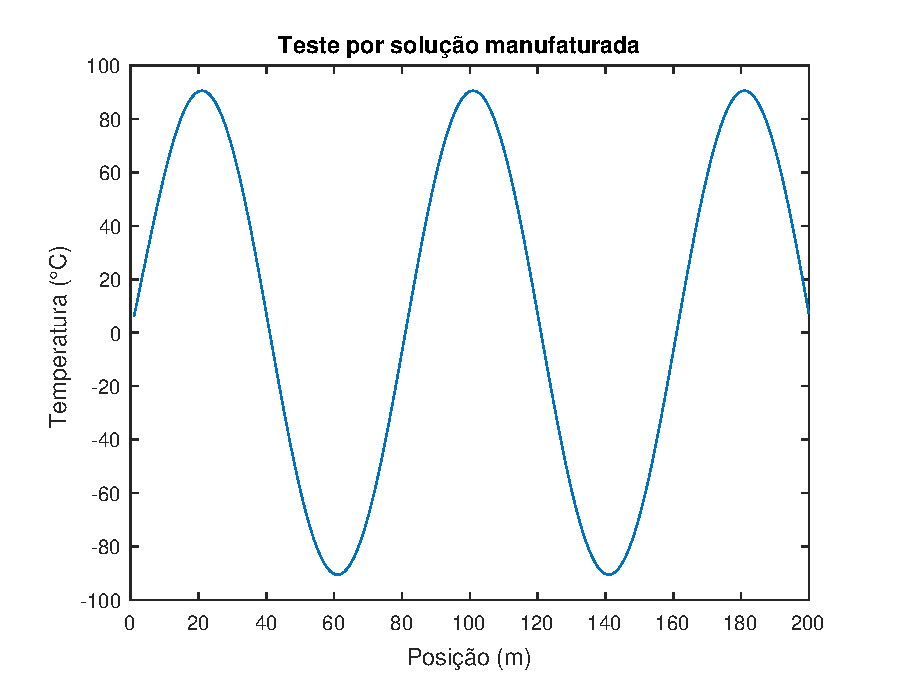
\includegraphics[width=.99\linewidth]{sol_manufaturada_convergindo}
		\caption{Solução numérica convergindo}
	\end{subfigure}
	\caption{Diferentes etapas do teste por solução manufaturada}
	\label{fig:diverge_sol_manufaturada_expl}
\end{figure}

Montando tabela com erros médios para variação no passo de tempo, obtivemos os seguintes erros globais ao executar uma simulação do início ao fim (parâmetros usados estão em parameters\_exact\_senoid.mat e resultados podem ser vistos executando show\_explicit\_error.m):

\begin{table}[htb]
\begin{center}
		\begin{tabular}{|c|c|c|}\hline
			Passo no tempo & Erro asocciado \\\hline
			5.000000e-04 & 3.082351e+04 \\\hline
			2.500000e-04 & 2.818915e-01 \\\hline
			1.250000e-04 & 2.127182e-01 \\\hline
			6.250000e-05 & 1.787781e-01 \\\hline
			3.125000e-05 & 1.621413e-01 \\\hline
			1.562500e-05 & 1.540372e-01 \\\hline
			7.812500e-06 & 1.501008e-01 \\\hline
			3.906250e-06 & 1.492907e-01 \\\hline
			1.953125e-06 & 1.504369e-01 \\\hline
		\end{tabular}
\caption{Erros globais do método explícito}
\end{center}
\end{table}

O primeiro valor corresponde a uma configuração onde o método divergiu. Para as outras, observamos que o método tende à solução exata. No entanto, diminuindo mais $\Delta t$, seu erro não continuou caindo, provavelmente devido a erros da discretização no espaço (o erro de truncação local é da ordem $O(\Delta t + \Delta x^2)$, como indicado na seção ``Métodos Numéricos'', não dependendo apenas do tempo e tendo algum erro mesmo para $\Delta t$ muito pequeno).

O erro de truncação local observado após um passo vale:

\begin{table}[htb]
\begin{center}
		\begin{tabular}{|c|c|c|c|}\hline
			Passo no tempo & Erro de truncação local & Razão entre erros (r) & $log_2$(r) \\\hline
			6.250000e-05 & 3.931024e-03 & - & - \\\hline
			3.125000e-05 & 1.968537e-03 & 1.9969 & 0.9978\\\hline
			1.562500e-05 & 9.850251e-04 & 1.9985 & 0.9989 \\\hline
			7.812500e-06 & 4.927017e-04 & 1.9992 & 0.9994\\\hline
			3.906250e-06 & 2.463981e-04 & 1.9996 & 0.9997\\\hline
			1.953125e-06 & 1.232109e-04 & 1.9998 & 0.9999\\\hline
			9.765625e-07 & 6.160840e-05 & 1.9999 & 0.9999\\\hline
			4.882813e-07 & 3.080494e-05 & 2.0000 & 1.0000 \\\hline
			2.441406e-07 & 1.540265e-05 & 2.0000 & 1.0000 \\\hline
			1.220703e-07 & 7.701373e-06 & 2.0000 & 1.0000 \\\hline
			6.103516e-08 & 3.850698e-06 & 2.0000 & 1.0000 \\\hline
			3.051758e-08 & 1.925352e-06 & 2.0000 & 1.0000 \\\hline
		\end{tabular}
\caption{Erros de truncação local do método explícito}
\end{center}
\end{table}

O método mostra ordem um no erro de truncação local para $\Delta t$. Passamos a escolher apenas intervalos onde o método converge. Convergência foi testada pela diferença máxima entre temperatura máxima e mínima (se maior que $10^5$, assume-se que o método está divergindo). Apenas um pequeno intervalo de $\Delta x$ mostrou convergência com os parâmetros escolhidos.

\begin{table}[htb]
\begin{center}
		\begin{tabular}{|c|c|c|c|}\hline
			Subdivisões do espaço & Erro de truncação local & Razão entre erros (r) & $log_2$(r) \\\hline
			128 & 1.48E-01 & - & - \\\hline
			64 & 2.96E-01 & 1.9928891764 & 0.9949 \\\hline
			32 & 5.83E-01 & 1.9699041496 & 0.9781 \\\hline
			16 & 1.09E+00 & 1.8742529782 & 0.9063 \\\hline
			8 & 1.56E+00 & 1.4303795961 & 0.5164 \\\hline
			4 & 9.69E+00 & 6.2020540534	& 2.6327 \\\hline
			2 & 4.26E+01 & 4.3980563901	& 2.1369 \\\hline
		\end{tabular}
\caption{Erros de truncação local do método explícito}
\end{center}
\end{table}

Podemos observar que o erro global do método tende à ordem 1 para número de subdivisões grande o suficiente, indicando erro de truncação local de ordem 2. Realizamos algumas simulações e observamos os resultados:

\begin{figure}[H]
	\centering
		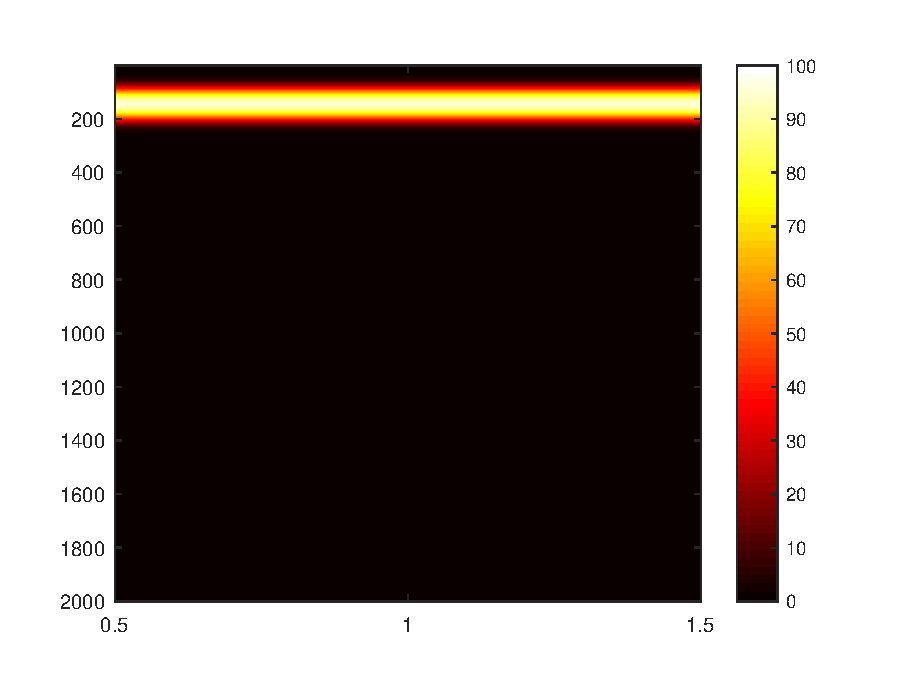
\includegraphics[height=10cm]{convergindo}
		\caption{Solução convergindo, parâmetros de Cobre e fonte de calor no topo}
\end{figure}

O fluxo foi desenhado calculando o gradiente e usando a função quiver(), que desenha um conjunto de setas. Na seguinte figura, as setas se sobrepõe e dificultam um pouco a visualização, mas observando a imagem original percebemos que as setas apontam para fora da região mais quente.

\begin{figure}[H]
	\centering
		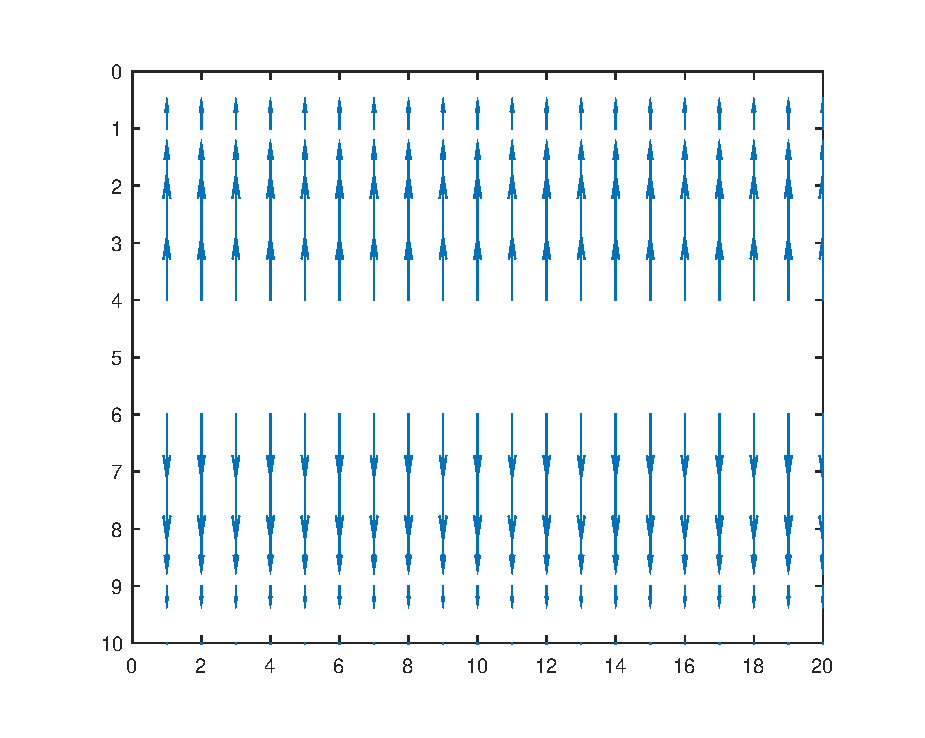
\includegraphics[height=10cm]{fluxo}
		\caption{Fluxo de calor}
\end{figure}

Testamos a implementação explícita para um plano. O estado do sistema é mantido em uma matriz nxn. A cada passo, a matriz é expandida em um vetor $n^2$x1, que será multiplicado por uma matriz com elementos nulos em todas as posições, exceto nos seus vizinhos (duas diagonais vizinhas às principais e duas diagonais distantes n elementos da principal, posição onde se encontram o bloco superior e inferior da placa). Iniciamos com uma matriz contendo um quadrado central mais quente. Pudemos observar alguns fenômonos do calor claramente (fluxo na interface entre as partes quente e fria e equilíbrio no interior).

\begin{figure}[H]
	\centering
	\begin{subfigure}{.5\textwidth}
		\centering
		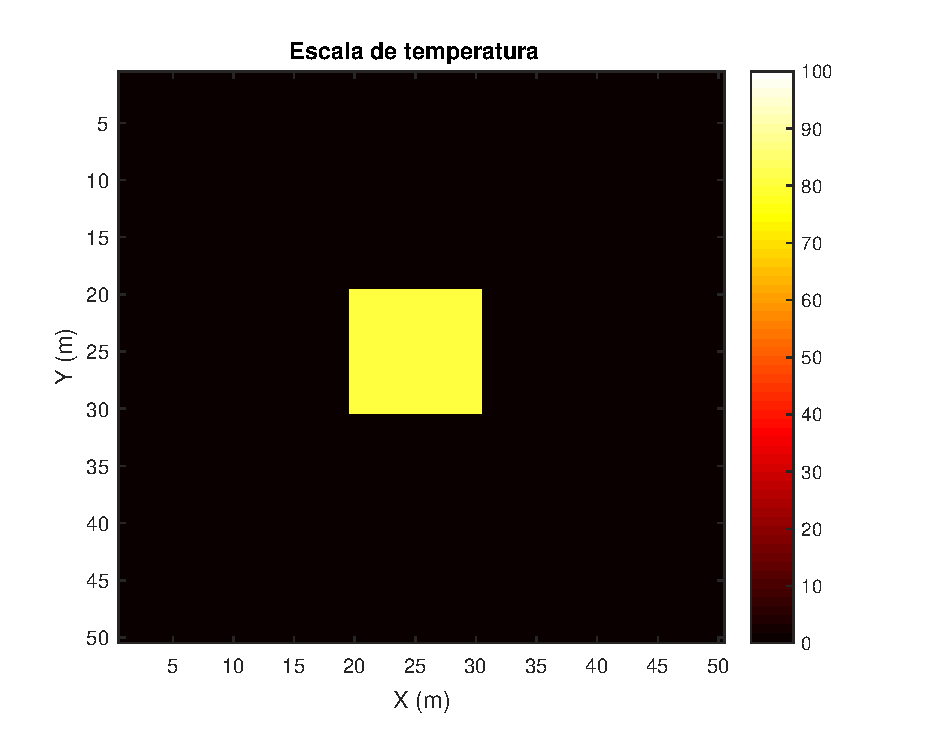
\includegraphics[width=.99\linewidth]{plano_inicial}
		\caption{Estado inicial}
	\end{subfigure}%
	\begin{subfigure}{.5\textwidth}
		\centering
		\includegraphics[width=.99\linewidth]{plano_fluxo_inicial}
		\caption{Fluxo inicial}
	\end{subfigure}
	\caption{Estado inicial da simulação realizada em plano}
\end{figure}

Após um segundo, temos:

\begin{figure}[H]
	\centering
	\begin{subfigure}{.5\textwidth}
		\centering
		\includegraphics[width=.99\linewidth]{temp_placa_segundos}
		\caption{Temperatura em um segundo simulado}
	\end{subfigure}%
	\begin{subfigure}{.5\textwidth}
		\centering
		\includegraphics[width=.99\linewidth]{fluxo_placa_segundos}
		\caption{Fluxo após um segundo simulado}
	\end{subfigure}
	\caption{Estado inicial da simulação realizada em plano}
\end{figure}

Apresentamos agora um método implícito, absolutamente estável. Tomando a equação $\frac{\partial u(x, t)}{\partial t} = \alpha \frac{\partial^2 u(x, t)}{\partial x^2} + w(x)$ e substituindo $\frac{\partial u(x, t)}{\partial t}$ pela diferença na temperatura entre dois passos dividido por $\Delta t$ e a segunda derivada pela aproximação deduzida na seção ``Métodos Numéricos'', temos:

\[
\frac{u(x, t + \Delta t) - u(x, t)}{\Delta t} - \alpha \frac{u(x - \Delta x, t) - 2 u(x, t) + u(x + \Delta x, t)}{\Delta x^2} = 0
\]

De onde obtemos a seguinte relação, onde A é a mesma matriz da resolução explícita:

\[
A * u(x, t + \Delta t) \approx u(x, t)
\]

Como A é tridiagonal, aplicaremos o algoritmo de Thomas para resolver o sistema. Testamos com passos de tempo largos e a simulação convergiu. Para variar o teste, começamos com estado inicial da barra aquecida em uma região próxima ao topo e uma fonte de calor no centro da barra. Esperamos que o calor concentrado na região aquecida inicialmente se disperse e surja um gradiente partindo do centro da barra.

\begin{figure}[H]
	\centering
	\begin{subfigure}{.5\textwidth}
		\centering
		\includegraphics[width=.99\linewidth]{implicito_temp_inicio}
		\caption{Temperatura}
	\end{subfigure}%
	\begin{subfigure}{.5\textwidth}
		\centering
		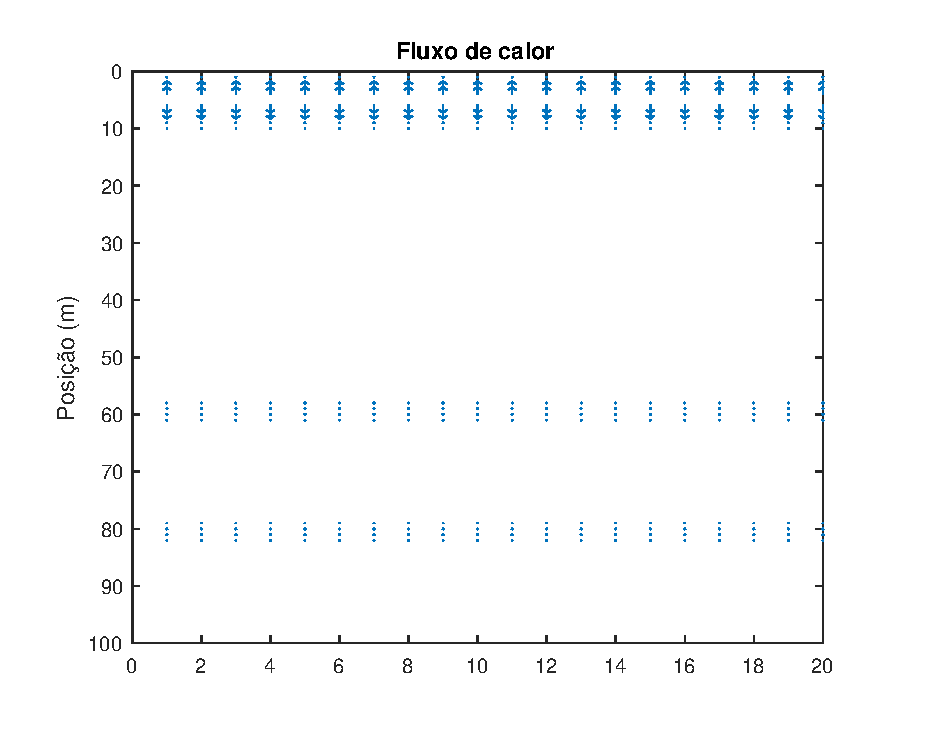
\includegraphics[width=.99\linewidth]{implicito_fluxo_inicio}
		\caption{Fluxo}
	\end{subfigure}
	\caption{Estado após uma iteração do modelo implícito para barra}
\end{figure}

\begin{figure}[H]
	\centering
	\begin{subfigure}{.5\textwidth}
		\centering
		\includegraphics[width=.99\linewidth]{implicito_temp_real_inicio}
		\caption{Temperatura}
	\end{subfigure}%
	\begin{subfigure}{.5\textwidth}
		\centering
		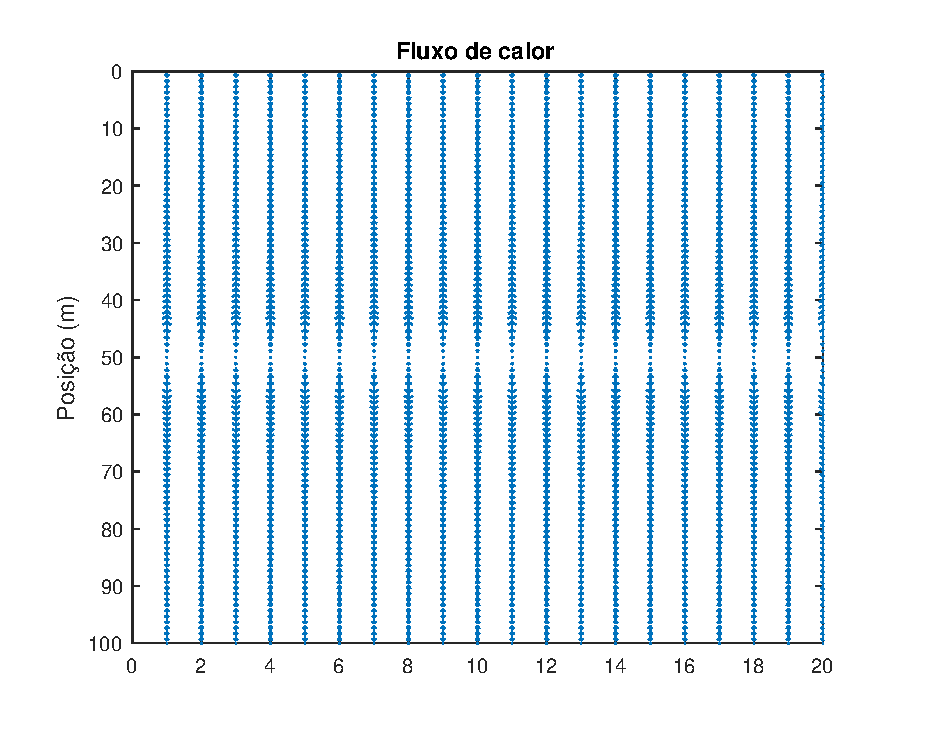
\includegraphics[width=.99\linewidth]{implicito_fluxo_fim}
		\caption{Fluxo}
	\end{subfigure}
	\caption{Estado para o qual o sistema convergiu}
\end{figure}

Por fim, calculamos um spline para aproximar uma função contínua passando pelos pontos que a simulação gerou. Testamos a função spline do MATLAB em uma função do terceiro grau usando condições de contorno (segunda derivada nas bordas) do polinômio. A função deve retornar os mesmos coeficientes da função. Como MATLAB não retorna diretamente os coeficientes do polinômio, mas realiza um deslocamento de cada intervalo para calcular \cite{splines}, verificamos manualmente os coeficientes retornados e eles eram os mesmos do polinômio. Fizemos também um programa que calcula pontos intermediários aos pontos do polinômio dados à função splines e compara com o valor real e os erros foram negligíveis (da ordem de $10^{-15}$):

\begin{verbatim}
function test_spline()
%TEST_SPLINE Testa spline aplicando em um polinômio do terceiro grau
%com condições de contorno (segunda derivada nos extremos) iguais à do
%polinômio
	x = 0:1:10;

	y = [2	x .* x .* x + x .* x + x	62];

	pp = spline(x, y(2:end-1));
	pp.coefs
	x = 0:0.1:10;

	error = ppval(pp, x) - (x .* x .* x + x .* x + x);

	display(mean(error));
end
\end{verbatim}

Tomamos o resultado da última simulação e aplicamos splines para encontrar uma solução contínua.

\begin{figure}[H]
	\centering
		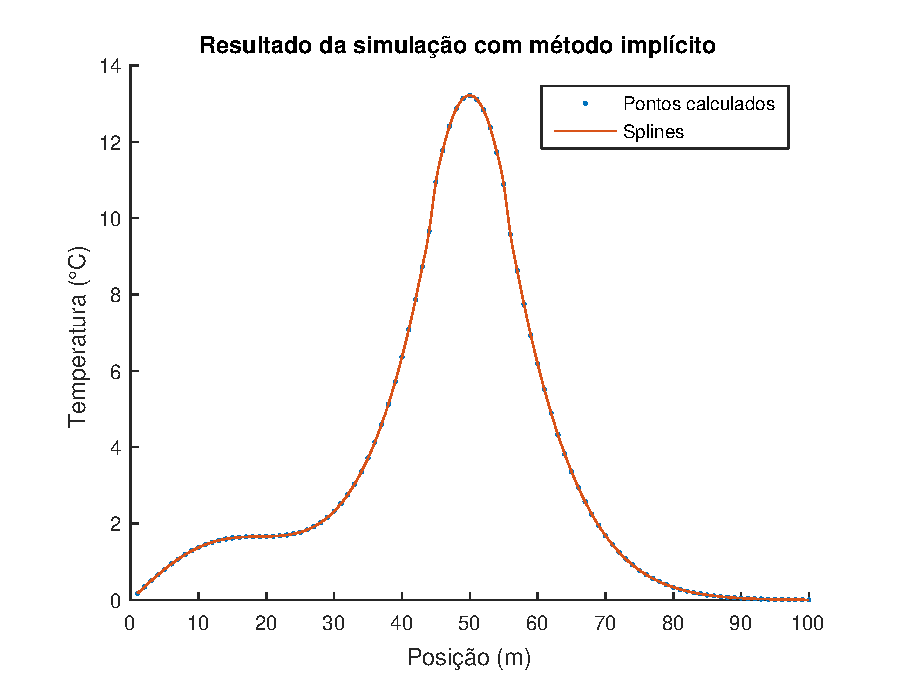
\includegraphics[height=10cm]{splines2}
		\caption{Solução encontrada e spline}
\end{figure}

\section{Conclusões}
Pudemos observar diferentes métodos de simular o mesmo fenômeno para 1 ou 2 dimensões. Vimos a dificuldade em utilizar o método condicionalmente convergente, que necessita de escolhas bastante restritas de passos de tempo pequenos para convergir. Em simulações com o método absolutamente convergente pudemos escolher passos de tempo muito maiores e resultados foram muito mais rápidos. Aplicamos muitos métodos da disciplina e treinamos o que aprendemos em aula.

\vspace{5mm}
{\bf{Agradecimentos}} Agradeçemos ao professor Alexandre Roma pelo apoio e incentivo ao trabalho.

\bibliographystyle{plain}
\bibliography{bibliografia}

\end{document} %finaliza o documento
